\subsection{Nouvelle manière de compter}
Suite à la réunion du 18 Juillet, on a décide de ne plus compter avec une fenêtre glissante. En effet cette façon générer des redondances dans la matrice de fréquences en kmers. Pour 
cela l'utilisateur à le choix de fournir son propre décalage (en nucléotide) sinon le programme utilise un décalage égale à 20\% de la taille de la fenêtre.

\subsection{Optimisation}
Dans un premier temps le programme à été revu pour prendre en compte ce décalage mais sans optimisation. L'optimisation consisterais à ne compter que les nouveau kmers lors du décalage de la fenêtre. Cette astuce était utilisée dans la version précédente. Mais étant que le décalage était égale à 1 nucléotides, une variable était suffisante pour mémoriser le kmer qui "sortait" de la nouvelle fenêtre comparé à la fenêtre précédente. On copiait ainsi la ligne de fréquence de la fenêtre précédente, on décrémenter la fréquence du kmer qui "sortait" et on calculait le nouveau kmer qui "entrait".
\\

Avec un décalage égale à $n$, on a $n$ kmer qui "sort" et $n$ nouveaux kmer à compter (entrant). Pour se faire on se propose d'utiliser deux tampons: 
\\
\begin{itemize}
 \item[.] $courant$: correspondant à la ligne de comptage actuel, pour une fenêtre donnée.
 \item[.] $precedent$: correspondant à la ligne de comptage pour la fenêtre précédente.
\end{itemize}
~\\

Ces tampons ont la même taille que le nombre de kmer présent dans la fenêtre, soit $f-k+1$ si $f$ est la taille de la fenêtre et $k$ la taille du kmer. Ainsi lors qu'on compte une toute première fois cela permet d'initialiser le tampon courant et de mémoriser tous les kmers rencontrés. Lorsqu'on passe à la fenêtre suivante si on effectue un décalage de $d$ nucléotides, il suffit donc:
\\
\begin{itemize}
 \item[.] D'intervertir les deux tampons
 \item[.] De copier les bonnes parties dans le nouveau tampon, courant
 \item[.] Calculer les nouveaux kmers entrant et sauvegarder dans le tampon courant.
\end{itemize}
~\\

On obtient donc les kmers rencontrés, et on augmente dans le tableau de fréquence par rapport au tampon courant. Voir figure \ref{decalage} pour illustration, avec un kmer=\#\#\#, une fenêtre de taille 7 et un décalage $d=2$.

\begin{figure}[H]
\begin{center}
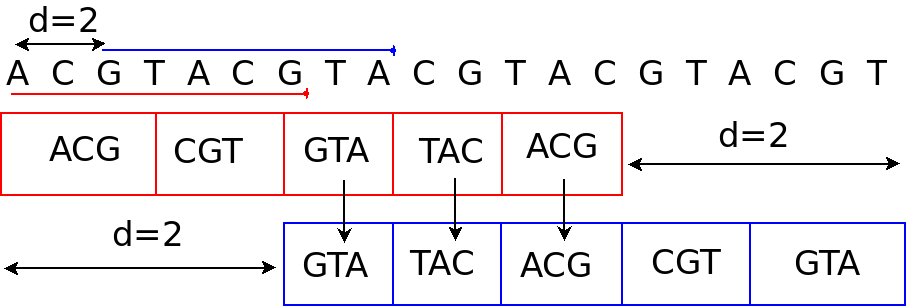
\includegraphics[scale=0.4]{./../img/decalage.png}
\caption[Principe du décalage]{\label{decalage}Principe du décalage avec une fenêtre de taille 7 et un tri-mers}
\end{center}
\end{figure}
~\\

Même si les tests sont ok et les tableaux de fréquences corrects. Il y a des cas où valgrind détecte des erreurs au niveau des ces buffers. D'autre erreurs par ailleurs sont également détecté par valgrind. L'objectif principal avant de continuer et d'éliminer toutes ces erreurs afin de continuer sur un programme "propre".
